\documentclass{article}
\usepackage[utf8]{inputenc}
\usepackage{amsmath}
\usepackage{braket}
\usepackage{gensymb}
\usepackage{amssymb}
\usepackage{natbib}
\usepackage{graphicx}
\usepackage{listings}
\usepackage{color}
\usepackage{tikz}
\usepackage{multicol}
\usetikzlibrary{arrows}
\usepackage{float}
\restylefloat{figure}

\usepackage[figurename=Figure]{caption}

\definecolor{codegreen}{rgb}{0,0.6,0}
\definecolor{codegray}{rgb}{0.5,0.5,0.5}
\definecolor{codepurple}{rgb}{0.58,0,0.82}
\definecolor{backcolour}{rgb}{0.95,0.95,0.92}
 
\lstdefinestyle{mystyle}{
    backgroundcolor=\color{backcolour},   
    commentstyle=\color{codegreen},
    %keywordstyle=\color{magenta},
    keywordstyle=\color{blue},
    numberstyle=\tiny\color{codegray},
    stringstyle=\color{codepurple},
    basicstyle=\footnotesize,
    breakatwhitespace=false,         
    breaklines=true,                 
    captionpos=b,                    
    keepspaces=true,                 
    %numbers=left,                    
    numbersep=5pt,                  
    showspaces=false,                
    showstringspaces=false,
    showtabs=false,                  
    tabsize=4
}
 
\lstset{style=mystyle}
\lstset{
    language=Erlang,
    mathescape=true
}
\usepackage{hyperref}
\hypersetup{
    colorlinks=true,
    linkcolor=blue,
    filecolor=magenta,      
    urlcolor=cyan,
}

\title{FYS2130 - Project}
\author{Candidate - 15266}
\date{April 2018}

\begin{document}

\maketitle

\section*{Problems}

\subsection*{Problem 1}
We are asked to solve the equation
\begin{equation}
ma(t) + kx(t) = 0,
\end{equation}
numerically using the Runge-Kutta 4 method where we have written the code ourself. We start by setting up an expression we can feed into our function, which is basicly just to solve for $a$ which yields
\begin{equation}
a(t) = -\frac{k}{m}x(t).
\end{equation}
Using the constants and initial conditions given in the problem, $x(0) = 1$ and $v(0) = 0$ produces an elipse as \ref{figure_1} shows. \ref{figure_2} shows plots of the energy as the particle moves, whichs shows the energy is constant as expected. Because the total energy is constant, we thus have have
\begin{equation}
E_{tot} = E_k + E_p = \frac{1}{2}mv^2 + \frac{1}{2}kx^2 = C,
\end{equation}
where C is a constant. This is the equation for an elipse. Changing the initial conditions only will always produce an elipse.
\begin{figure}[H]
\centering
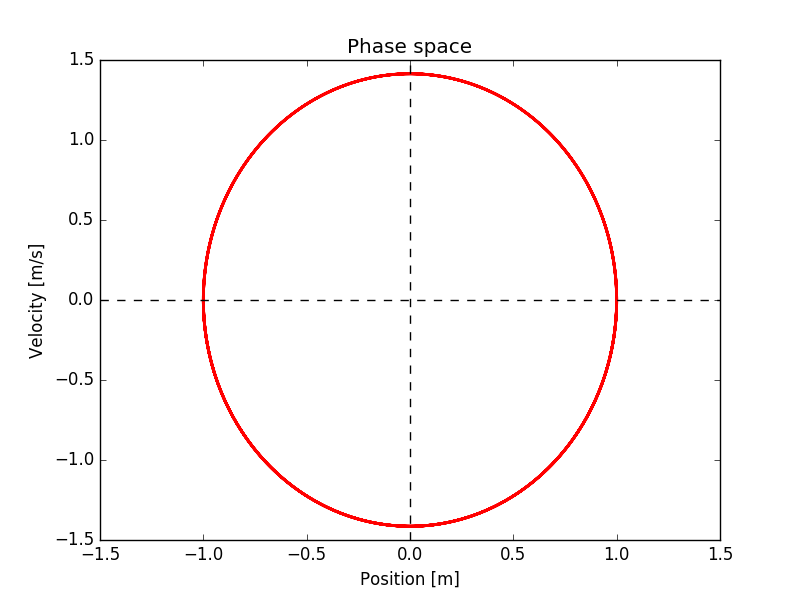
\includegraphics[width=0.75\textwidth]{problem_1_1}\label{figure_1}
\caption{Phase diagram of a harmonic oscilator.}
\label{fig:problem_b_contour_fig}
\end{figure}
\begin{figure}[H]
\centering
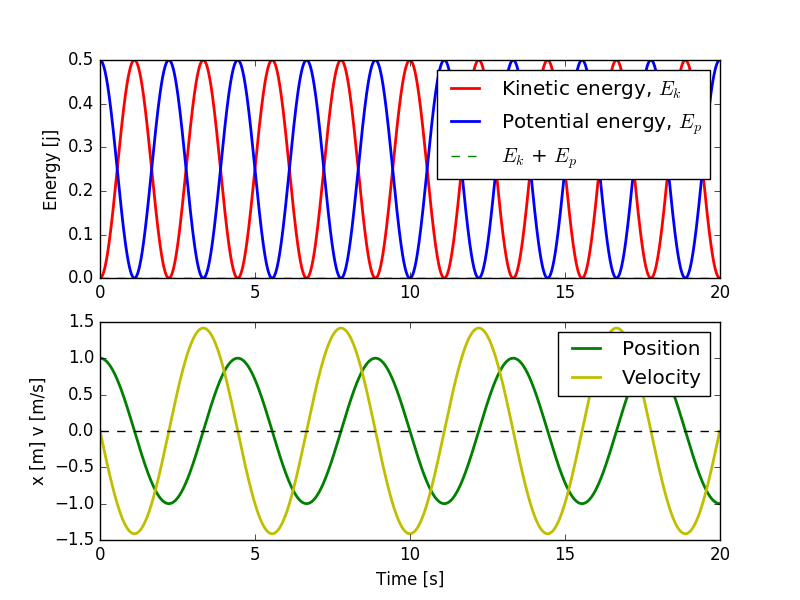
\includegraphics[width=0.75\textwidth]{problem_1_2}
\caption{Energy for harmonic oscillator.}
\label{fig:problem_b_contour_fig}
\end{figure}

\subsection*{Problem 2}
We will now include damping which yields
\begin{equation}
a(t) = -\frac{k}{m}x(t) - \frac{b}{m}v(x).
\end{equation}
\begin{figure}[H]
\centering
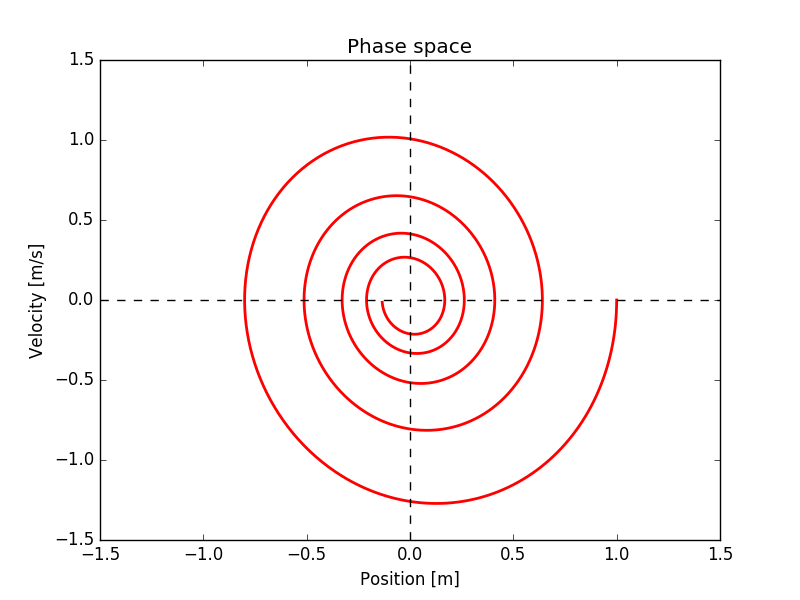
\includegraphics[width=0.75\textwidth]{problem_2_1}\label{figure_1}
\caption{Phase diagram of a harmonic oscilator.}
\label{fig:problem_b_contour_fig}
\end{figure}
\begin{figure}[H]
\centering
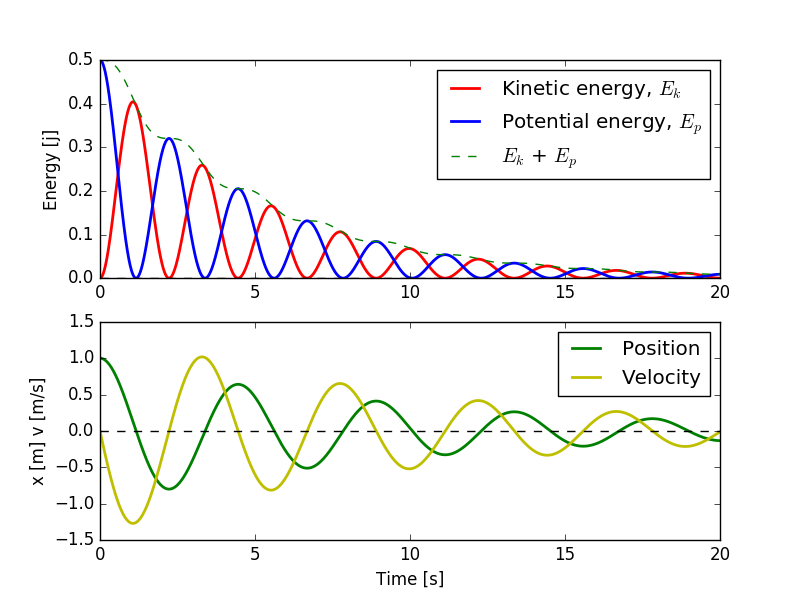
\includegraphics[width=0.75\textwidth]{problem_2_2}
\caption{Energy for damped harmonic oscillator.}
\label{fig:problem_b_contour_fig}
\end{figure}

\subsection*{Problem 3}
% https://www.youtube.com/watch?v=iQoAbO_xlFs
% http://math.colgate.edu/~wweckesser/math308Fall02/handouts/ForcedHarmonicOsc.pdf
We are asked to solve the following differential equation
\begin{equation}
m\ddot{x}(t) + kx(t) = F_D\cos{\omega_Dt},
\end{equation}
analytically. This type of equation is called \textit{the Periodically Forced Harmonic Oscillator}. $b=0$, which means this is a undamped system. This is a second order nonlinear, nonhomogeneous differential equation. A differential equation on this form is solved by adding the solution of the homogeneous and the solution of the particular solution. By the method of undetermined coefficients, the general solution is
\begin{equation}
x(t) = c_1\cos{(\omega_0t)} + c_2\sin{(\omega_0t)} + \frac{F_D}{m(\omega_D^2 - \omega_0^2)}\cos{(\omega_D t)},
\end{equation}
which yields
\begin{equation}
\dot{x}(t) = -c_1\omega_0\sin{(\omega_0t)} + c_2\omega_0\sin{(\omega_0t)} - \omega_D\frac{F_D}{m(\omega_D^2 - \omega_0^2)}\sin{(\omega_D t)},
\end{equation}
where $\omega_0 = \sqrt{k/m}$ is the \textit{natural frequency} of the undamped harmonic oscillator.
We need to solve this for the initial conditions $x(0) = 2.0$ and $\dot{x}(0) = 0.0$, namely
\begin{equation}
x(0) = c_1 + \frac{F_D}{m(\omega_D^2 - \omega_0^2)} = 2.0 \rightarrow c_1 = 2.0 - \frac{F_D}{m(\omega_D^2 - \omega_0^2)} \ \text{and}
\end{equation}
\begin{equation}
\dot{x}(0) = c_2\omega_0\cos{(\omega_0t)} = 0.0 \rightarrow c_2 = 0.0.
\end{equation}
Using the initial conditions given, we get the following plots
\begin{figure}[H]
\centering
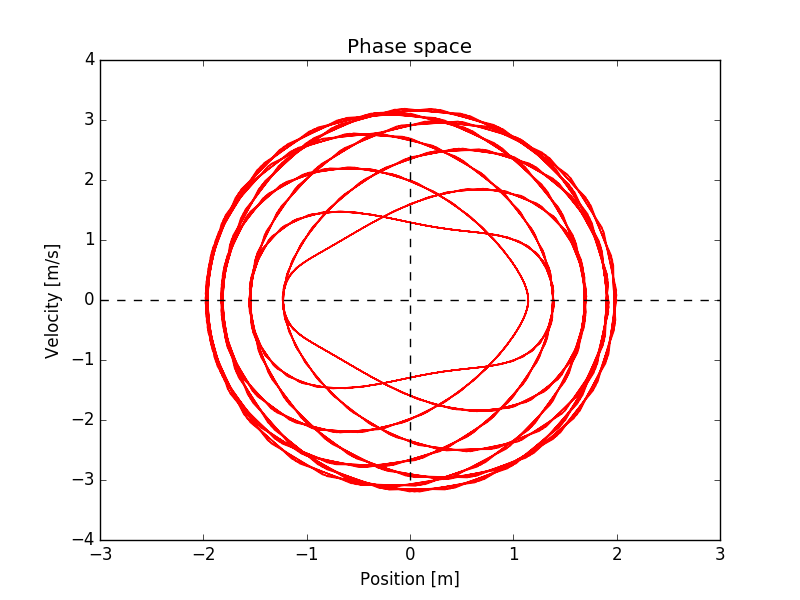
\includegraphics[width=0.75\textwidth]{problem_3_1}\label{figure_1}
\caption{Phase diagram of a harmonic oscilator.}
\label{fig:problem_b_contour_fig}
\end{figure}
\begin{figure}[H]
\centering
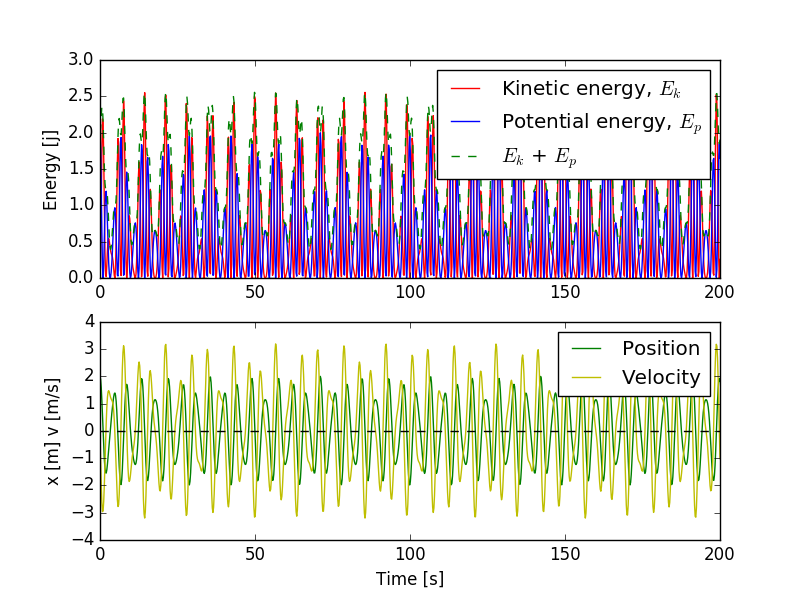
\includegraphics[width=0.75\textwidth]{problem_3_2}
\caption{Energy for damped harmonic oscillator.}
\label{fig:problem_b_contour_fig}
\end{figure}



\subsection*{Problem 4}
\begin{figure}[H]
\centering
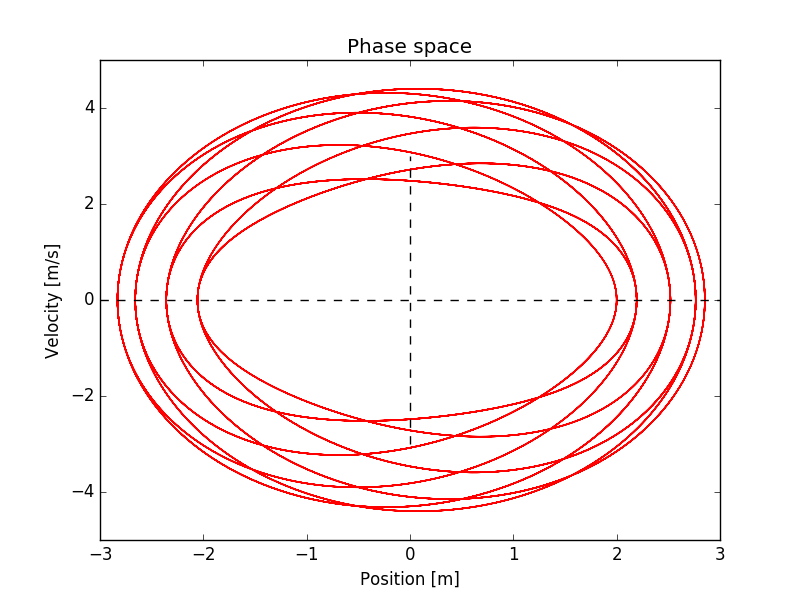
\includegraphics[width=0.75\textwidth]{problem_4_1_1}\label{figure_1}
\caption{Phase diagram of a harmonic oscilator.}
\label{fig:problem_b_contour_fig}
\end{figure}
\begin{figure}[H]
\centering
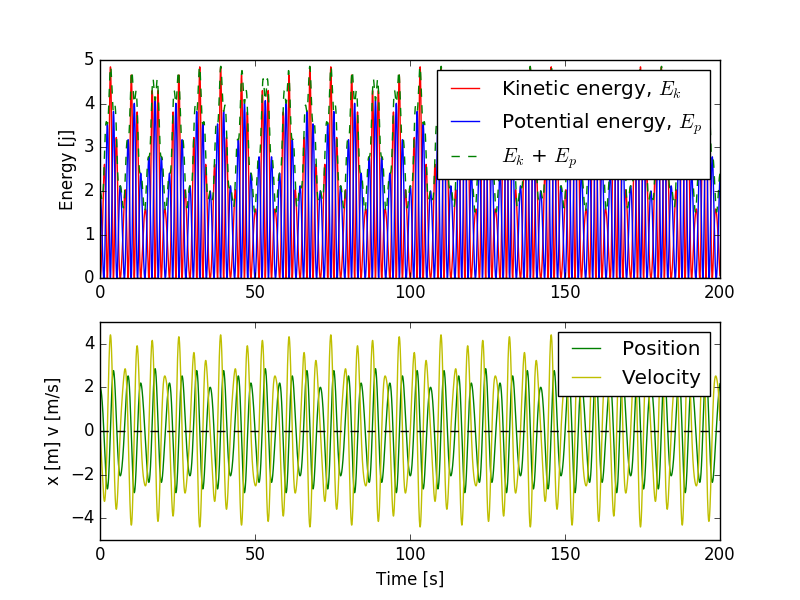
\includegraphics[width=0.75\textwidth]{problem_4_1_2}
\caption{Energy for damped harmonic oscillator.}
\label{fig:problem_b_contour_fig}
\end{figure}
\begin{figure}[H]
\centering
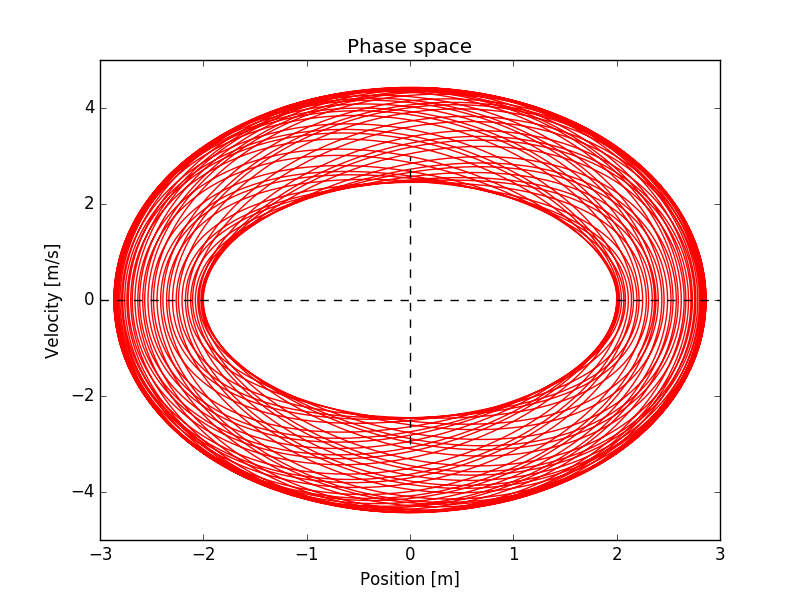
\includegraphics[width=0.75\textwidth]{problem_4_2_1}\label{figure_1}
\caption{Phase diagram of a harmonic oscilator.}
\label{fig:problem_b_contour_fig}
\end{figure}
\begin{figure}[H]
\centering
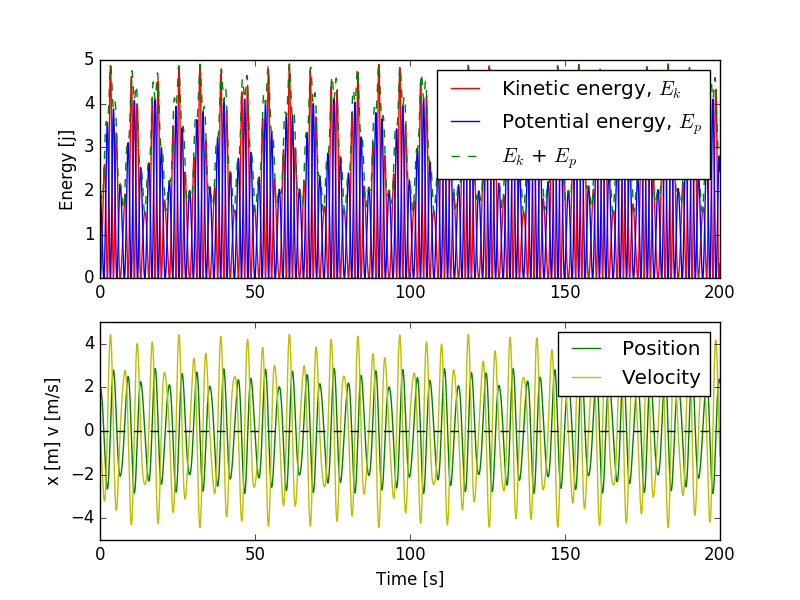
\includegraphics[width=0.75\textwidth]{problem_4_2_2}
\caption{Energy for damped harmonic oscillator.}
\label{fig:problem_b_contour_fig}
\end{figure}



\subsection*{Problem 5}
\begin{figure}[H]
\centering
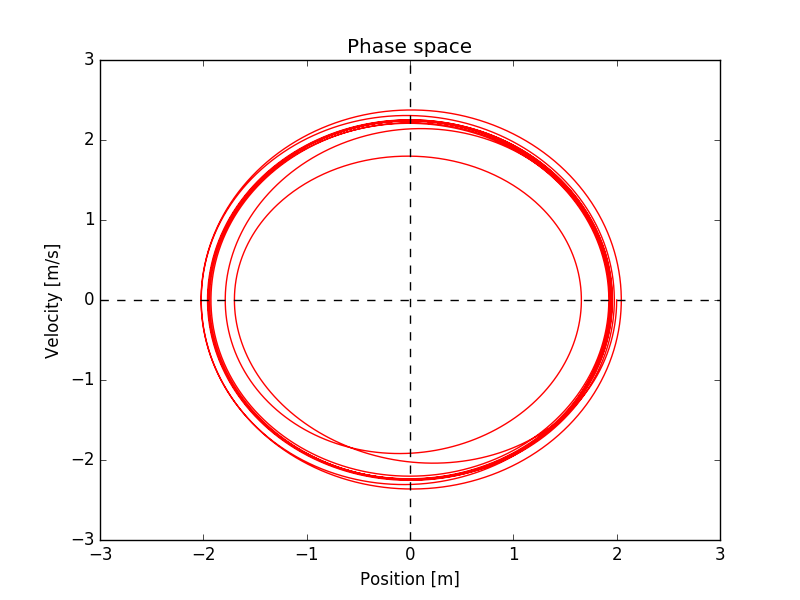
\includegraphics[width=0.75\textwidth]{problem_5_1}\label{figure_1}
\caption{Phase diagram of a harmonic oscilator.}
\label{fig:problem_b_contour_fig}
\end{figure}
\begin{figure}[H]
\centering
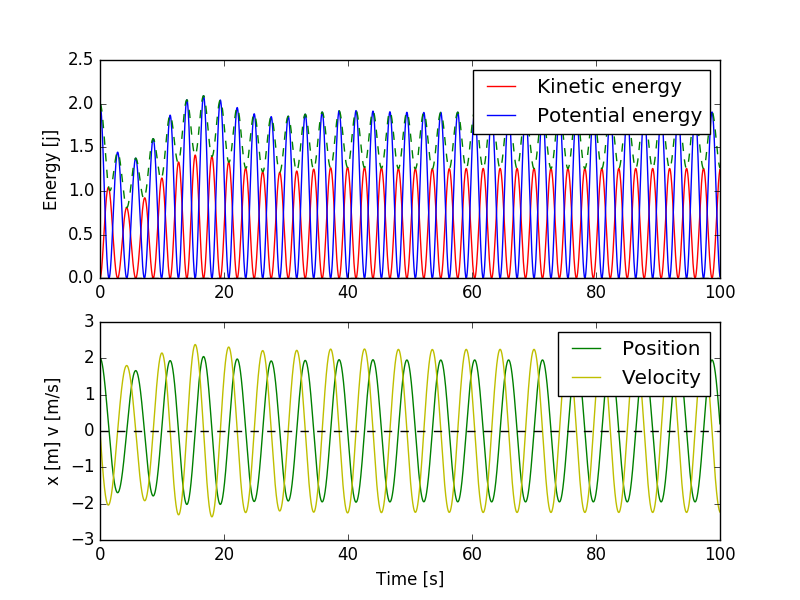
\includegraphics[width=0.75\textwidth]{problem_5_2}
\caption{Energy for damped harmonic oscillator.}
\label{fig:problem_b_contour_fig}
\end{figure}


\subsection*{Problem 6}
%\begin{figure}[H]
%\centering
%\includegraphics[width=0.75\textwidth]{problem_6_1}\label{figure_1}
%\caption{Phase diagram of a harmonic oscilator.}
%\label{fig:problem_b_contour_fig}
%\end{figure}
%\begin{figure}[H]
%\centering
%\includegraphics[width=0.75\textwidth]{problem_6_2}
%\caption{Energy for damped harmonic oscillator.}
%\label{fig:problem_b_contour_fig}
%\end{figure}


\subsection*{Problem 7}

\subsection*{Problem 8}

\subsection*{Problem 9}

\section*{Appendix}

\subsection*{Python code}
\hypertarget{pythonsourcecode}{}
\lstinputlisting[language=Python]{code.py}


\end{document}

